\documentclass{beamer}
\usetheme{Copenhagen}
\usecolortheme{whale}
\usefonttheme[onlymath]{serif}

\usepackage{setspace}
\usepackage{xcolor}
\usepackage{graphicx}
\usepackage{multimedia}
\usepackage{fontawesome}
\usepackage[most]{tcolorbox}
\usepackage{empheq}
\usepackage{fancybox}
\usepackage{annotate-equations}
\usepackage{tikz}
\usetikzlibrary{positioning, calc, shapes.geometric, shapes.multipart, 
	shapes, arrows.meta, arrows, 
	decorations.markings, external, trees}
\tikzstyle{Arrow} = [
thick, 
decoration={
	markings,
	mark=at position 1 with {
		\arrow[thick]{latex}
	}
}, 
shorten >= 3pt, preaction = {decorate}
]

\title[Does Machine Learning Work?]{Does Machine Learning Work?: Designing Better Simulation Studies for Inference}
\author[Zivich]{Paul Zivich \\~\\ Institute of Global Health and Infectious Diseases \\ University of North Carolina at Chapel Hill}

\setbeamercovered{transparent}
\setbeamertemplate{navigation symbols}{}  % gets rid of the dumb navigation symbols
\setbeamertemplate{page number in head/foot}{\insertframenumber}  % adds slide #
\setbeamertemplate{headline}{}

\AtBeginSection[]{
	\begin{frame}
		\vfill
		\centering
		\begin{beamercolorbox}[sep=8pt,center,shadow=true,rounded=true]{title}
			\usebeamerfont{title}\insertsectionhead\par%
		\end{beamercolorbox}
		\vfill
	\end{frame}
}

\begin{document}
	
\begin{frame}[plain]
	\centering
	\maketitle
\end{frame}

\begin{frame}{Problem}
	\centering
	\Large
	How can we \textit{know} our tools work as intended?
\end{frame}

\begin{frame}{Causal Inference}
	\textbf{Problem}: estimate the average causal effect (ACE)~\\
	\[\psi_{1-0} = E[Y^1] - E[Y^0]\]
	where $Y^a$ is the potential outcome under action $a$\\~\\
	\textbf{Data}: action ($A$), outcome ($Y$), and covariates ($W$) for $n$ units
\end{frame}

\begin{frame}{Identification of Causal Effects}
	Identification
	\begin{itemize}
		\item Express $\psi_{1-0}$ in terms of $W,A,Y$
		\item Causal consistency, conditional exchangeability, positivity
	\end{itemize}{\small ~\\}
	\begin{equation*}
		\begin{aligned}
			E[Y^a] = & \sum_{w} E[Y^a | W=w] \Pr(W=w) && \text{Total Exp} \\
			 = & \sum_{w} E[Y^a | A=a, W=w] \Pr(W=w)  && \text{Exch \& Pos}\\ 
			 = & \sum_{w} E[Y | A=a, W=w] \Pr(W=w)  && \text{Consistency}\\ 
		\end{aligned}
	\end{equation*}
	Hereafter assume identification assumptions are true\footnote[frame]{This is the best case, but could also be consider when not met}	
\end{frame}

\begin{frame}{Identification is \textit{Not} Enough\footnote[frame]{Maclaren \& Nicholson (2019). `What can be estimated? Identifiability, estimability, causal inference and ill-posed inverse problems' \textit{arXiv}}}
	Suppose $W$ is high-dimensional
	\begin{itemize}
		\item Continuous variable or many categorical variables
		\item $\Pr(A=a | W=w)$ and $E[Y | A=a, W=w]$
		\begin{itemize}
			\item Cannot nonparametrically estimate
			\item Informally,\footnote[frame]{This is the case asymptotically when $W$ is continuous} there will always be a $w$ with $A=0$ but no units with $A=1$ even as $n \rightarrow \infty$
			\item Common is all but the simplest applications 
		\end{itemize}
	\end{itemize}~\\
	To make progress, we use models
\end{frame}

\begin{frame}{Causal Effect Estimation with Models}
	Using models to estimate 
	\begin{itemize}
		\item Define a narrower set of distributions; $\mathcal{M}_\alpha$, $\mathcal{M}_\beta$
		\[\Pr(A=a | W=w; \alpha) = \pi_a(W; \alpha)\]
		\[E[Y | A=a, W=w; \beta] = m_a(W; \beta)\]
		\item Allows us to interpolate or extrapolate over sparsity
	\end{itemize}~\\~\\
	\begin{equation*}
		\eqnmarkbox[violet]{node1}{\hat{\psi}_a}
		=
		\frac{1}{n}
		\sum_{i=1}^{n}
		\eqnmarkbox[red]{node2a}{m_a(W_i; \hat{\beta})}
		+ 
		\frac{Y_i - 
			\eqnmarkbox[red]{node2b}{m_a(W_i; \hat{\beta})}}{
			\eqnmarkbox[blue]{node3}{\pi_a(W_i; \hat{\alpha})}
		}
	\end{equation*}
	\annotate[yshift=1.5em]{right}{node1}{AIPW}	
	\annotatetwo[yshift=1.25em]{label above}{node2a}{node2b}{Outcome process}
	\annotate[yshift=-0.5em]{below,left}{node3}{Propensity score}
\end{frame}

\begin{frame}{Causal Effect Estimation with Models}
	Use of models \textit{is not free}
	\begin{itemize}
		\item No model misspecification
		$$\Pr(A=a | W=w) \in \mathcal{M}_\alpha$$
		$$E[Y | A=a, W=w] \in \mathcal{M}_\beta$$
		\item Models include correct functional forms
		\begin{itemize}
			\item Interaction terms, variable transformations, etc.
		\end{itemize}
	\end{itemize}
	~\\
	Epidemiologists commonly use \textit{parametric} models
	\begin{itemize}
		\item Quite restrictive assumptions on functional forms
	\end{itemize}
\end{frame}

\begin{frame}{Causal Effect Estimation with Models\footnote[frame]{Coverage of parametric models not to scale}}
	\centering
	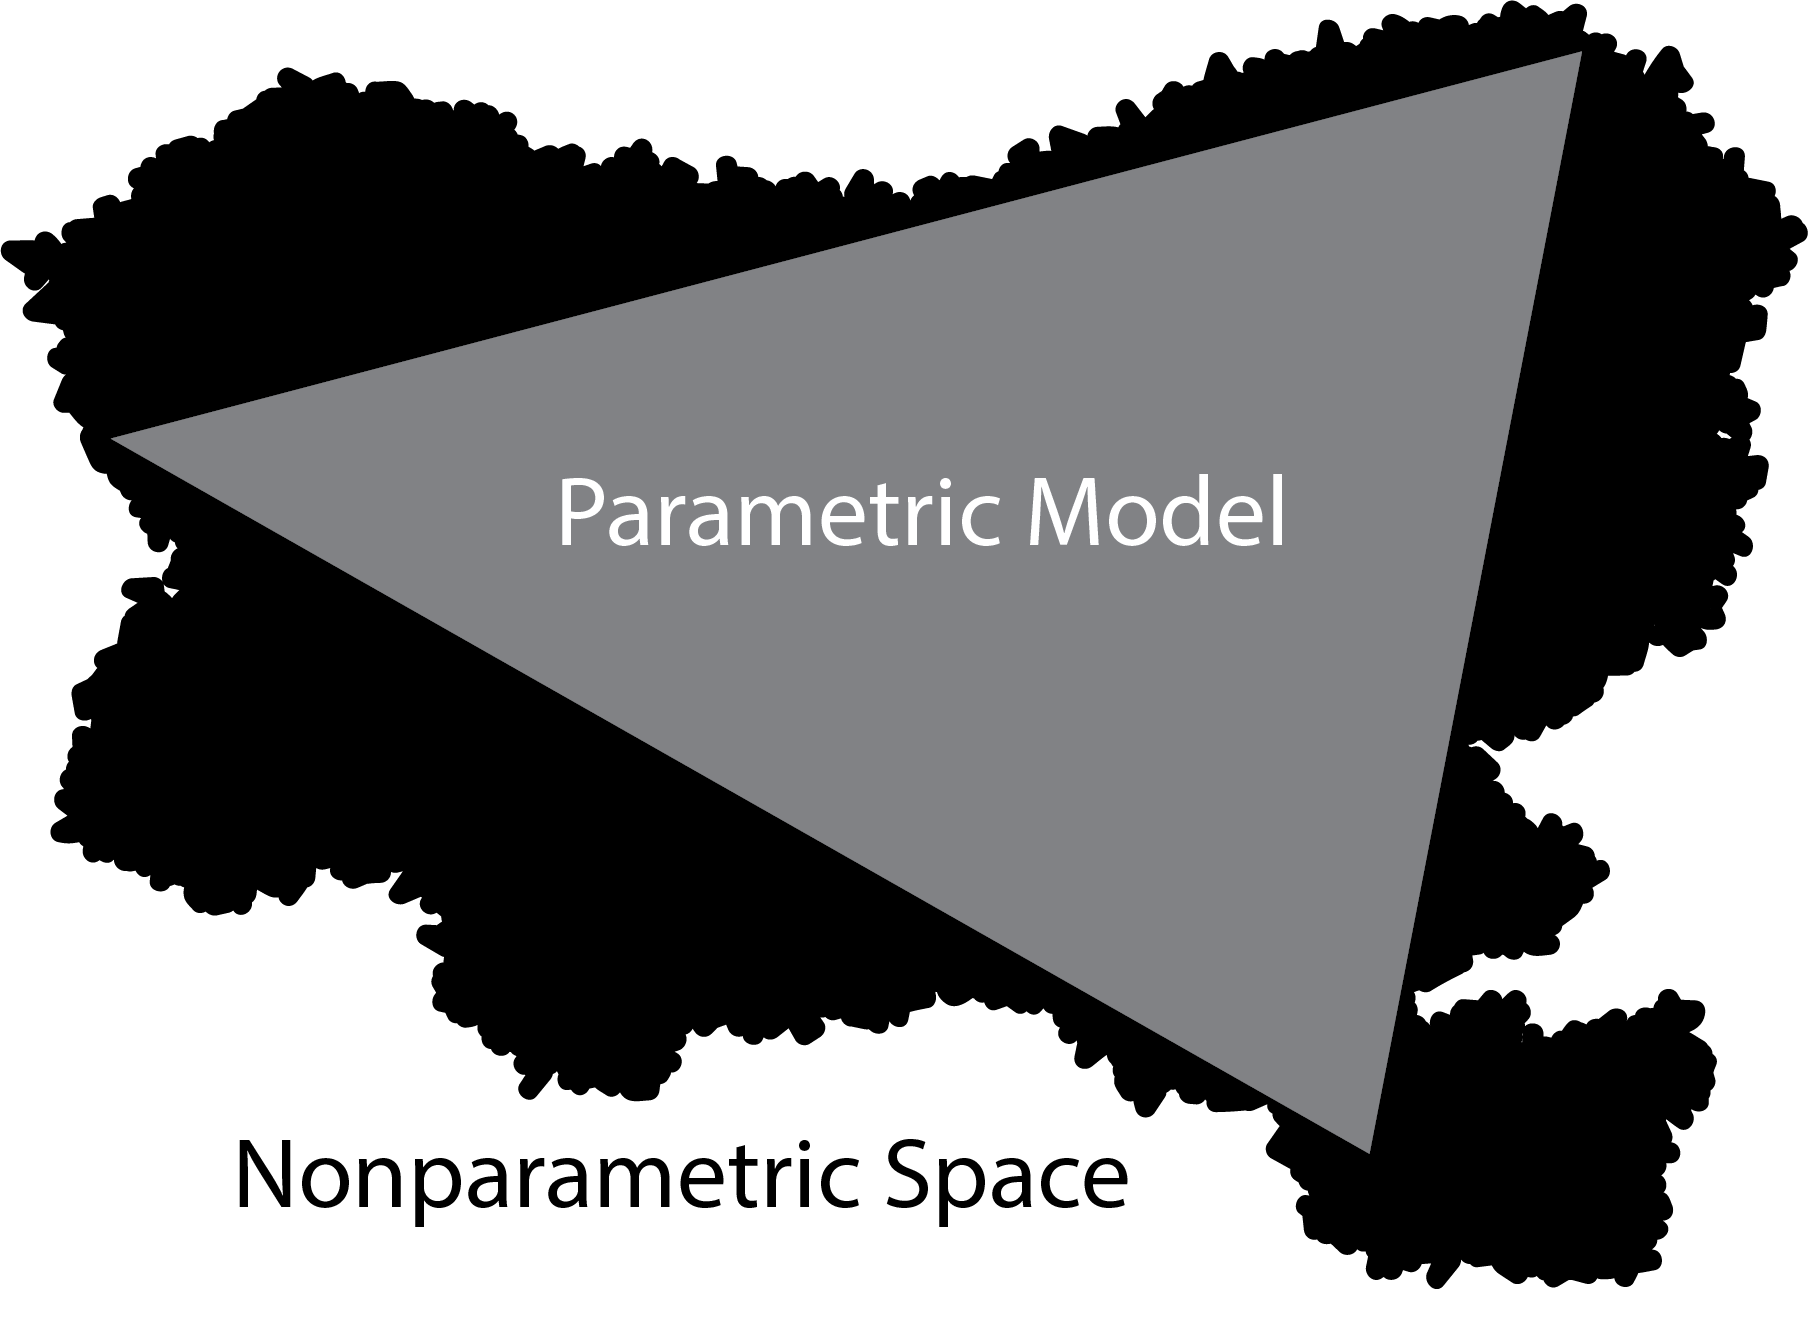
\includegraphics[width=0.85\linewidth]{parametric_model.png}
\end{frame}

\begin{frame}{The Promise of Machine Learning}
	The assumption of no model misspecification is worrisome
	\begin{itemize}
		\item Are parametric models flexible enough?
		\item Do epidemiologists specify them to that level of flexibility?
	\end{itemize}~\\
	Machine learning % \footnote[frame]{I still lack a clear definition that distinguishes the `usual' statistical methods from machine learning}
	\begin{itemize}
		\item More flexible than standard parametric approaches
		\begin{itemize}
			\item Captures a wider set of distributions
		\end{itemize}
		\item Removes some burden from the researchers
		\begin{itemize}
			\item May not need to specify interactions or non-linearities
		\end{itemize}
	\end{itemize}
\end{frame}

\begin{frame}{Causal Effect Estimation with Models\footnote[frame]{Coverage of ML models not to scale}}
	\centering
	\includegraphics[width=0.9\linewidth]{ml_model.png}
\end{frame}

\begin{frame}{But Does Machine Learning Work?}
	Does machine learning allow us to estimate causal effects we couldn't otherwise \textit{in practice}?
	\begin{itemize}
		\item Would a flexible penalized parametric model work similarly?
	\end{itemize}
	~\\~\\
	Does machine learning give us a `better' estimator for the ACE?
	\begin{itemize}
		\item Is the computational complexity worth it?
		\item Can I reasonably trust these black box algorithms?
	\end{itemize}
	~\\~\\
	Secondary questions: best practices for application
\end{frame}

\begin{frame}{Forms of Evidence to Consider}
	\centering\Large
	Mathematical Proof (deductive)
	\\~\\~\\
	Simulation (inductive)
\end{frame}

\begin{frame}{Mathematical Proof}
	Given a set of assumptions\footnote[frame]{Learn deductively rather than inductively}
	\begin{itemize}
		\item Does the tool work?
	\end{itemize}~\\
	Population inference
	\begin{itemize}
		\item Random sample of population
		\item Asymptotic results
		\begin{itemize}
			\item Behavior as $n \rightarrow \infty$
			\item Given large amounts of data, our method \textit{should} work
			\item If it doesn't, suspect for any realistic $n$
		\end{itemize}
	\end{itemize}
\end{frame}

\begin{frame}{Mathematical Proofs: Machine Learning}
	Key results\footnote[frame]{Reviewed in Zivich, Breskin, Kennedy (2023). `Machine Learning and Causal Inference'. In \textit{Wiley StatsRef}}
	\begin{itemize}
		\item Machine learning can capture a broader range of distributions
		\item Two concerns for machine learning application
		\begin{itemize}
			\item Statistical convergence rates
			\begin{itemize}
				\item Flexibility / convergence trade-off
				\item Solution: AIPW / TMLE
			\end{itemize}
			\item Complexity
			\begin{itemize}
				\item Limit complexity as to prevent over-fitting
				\item Solution: sample-splitting / cross-fitting
			\end{itemize}
		\end{itemize}
	\end{itemize}~\\
	But does this additional flexibility matters \textit{in practice}?
\end{frame}

\begin{frame}{Limits of Mathematical Proofs}
	Asymptotic results
	\begin{itemize}
		\item What can this tell us about practical application?
		\begin{itemize}
			\item Good asymptotic properties $\ne$ good in practice
			\item Finite-sample bias can be too large
		\end{itemize}
		\item Therefore not the full picture
	\end{itemize}
\end{frame}

\begin{frame}{Limits of Mathematical Proofs}
	``Such considerations reinforce the notion that (even if supporting theorems are available) great caution is needed in using a rule or method without extensive simulations to investigate the conditions under which it might be reasonable for practice. [...] 
	\\ ~[E]pidemiologic inference [...] may come to rely on computations and simulations tailored to the specifics of the study context, rather than rely solely on general results or methods"
	\footnote[frame]{Greenland (2012) `Commentary: Intuitions, Simulations, Theorems: The Role and Limits of Methodology' \textit{Epidemiology}}
\end{frame}

\begin{frame}{Simulation}
	\centering
	\includegraphics[width=0.95\linewidth]{simulation_flow.png}
	%Instead we can simulate
	%\begin{itemize}
	%	\item Generate some observations
	%	\item Apply estimator(s)
	%	\item Compare performance
	%\end{itemize}~\\	
	%Address the previous limitation of mathematical proofs
	%\begin{itemize}
	%	\item Assess performance in settings `closer' to applications
	%\end{itemize}~\\
	%But how can we get close to applications
	%\begin{itemize}
	%	\item Through the data generating mechanism
	%\end{itemize}
\end{frame}

\begin{frame}{Simulation: Parametric}
	\[W \sim \text{Normal}(\mu, \sigma)\]
	\[A \sim \text{Bernoulli}(\text{expit}(\alpha_0 + \alpha_1 W))\]
	\[Y \sim \text{Bernoulli}(\text{expit}(\beta_0 + \beta_1 A + \beta_2 W))\]
	~\\
	Limitations
	\begin{itemize}
		\item Idealized example 
		\begin{itemize}
			\item No reason to presuppose the world adheres to parametric models
			\item Too abstracted to be relevant to practice
		\end{itemize}
		\item An unfair comparison?
		\begin{itemize}
			\item May set up parametric models to succeed
			\item Machine learning looks less impressive
		\end{itemize}
	\end{itemize}
\end{frame}

%\begin{frame}{Example of the Issue with Super Learner}
%	Suppose the following simulation study
%	\begin{itemize}
%		\item Assess performance of super learner
%		\item Super learner
%		\begin{itemize}
%			\item[1] Linear regression
%			\item[2] Neural network
%			\item[3] Random forest
%		\end{itemize}
%		~\\
%		\item Assessing with a correctly specified linear regression model
%		\begin{itemize}
%			\item Less informative for cases where 
%		\end{itemize}
%		\item If linear regression is the correct model, can mislead us regarding performance in settings where parametric models are incorrect\footnote[frame]{Super learner has slightly slower convergence rates than root-$n$ when an included parametric model is correctly specified}
%	\end{itemize}
%\end{frame}

\begin{frame}{Simulation: Parametric\footnote[frame]{Zivich \& Breskin (2021) `Machine Learning for Causal Inference: On the Use of Cross-fit Estimators' \textit{Epidemiology}}}
	\centering
	\includegraphics[width=0.6\linewidth]{zivich_mechanisms.PNG}
\end{frame}

\begin{frame}{Simulation: Parametric\footnote[frame]{Naimi, Mishler \& Kennedy (2021) `Challenges in Obtaining Valid Causal Effect Estimates with Machine Learning Algorithms' \textit{Am J Epidemiol}}}
	\centering
	\includegraphics[width=0.8\linewidth]{naimi_mechanisms.PNG}
\end{frame}

\begin{frame}{Simulation: Plasmode}
	Plasmode simulations use a ``dataset that is created from natural processes but has some aspect of the data-generating model known"\footnote[frame]{Quote from Franklin et al. (2014) `Plasmode simulation for the evaluation of pharmacoepidemiologic methods in complex healthcare databases' \textit{Comput Stat Data Anal}}
	\begin{itemize}
		\item Tailored to a specific application
		\item Reference (truth) can be easily computed using known model
		\item Improvement over previous approach
	\end{itemize}~\\
	Limitations
	\begin{itemize}
		\item Use of a known model to generate the data
		\begin{itemize}
			\item Places us back in the same criticism 
		\end{itemize}
	\end{itemize}
\end{frame}

\begin{frame}{Simulation: Plasmode\footnote[frame]{Meng \& Huang (2021) `REFINE2: A tool to evaluate real-world performance of machine-learning based effect estimators for molecular and clinical studies' \textit{arXiv}}}
	\centering
	\includegraphics[width=0.9\linewidth]{meng_mechanisms.PNG}
\end{frame}

\begin{frame}{Beyond Plasmode Simulations}
	Generate simulation data where 
	\begin{itemize}
		\item Avoid simple parametric distributions
		\item But still easily compute the reference (true) ACE
	\end{itemize}~\\
	%Other desirable features
	%\begin{itemize}
	%	\item Mimic a specific application
	%	\item Automated
	%	\item Computationally efficient
	%\end{itemize}
\end{frame}

\begin{frame}{Beyond Plasmode Simulations}
	Credence\footnote[frame]{Parikh et al. (2022) `Validating causal inference methods. In International Conference on Machine Learning' \textit{PMLR}}
	\begin{itemize}
		\item Variational autoencoder neural networks
	\end{itemize}~\\~\\
	Wasserstein Generative Adversarial Neural Networks\footnote[frame]{Athey et al. (2021) `Using Wasserstein generative adversarial networks for the design of Monte Carlo simulations' \textit{Journal of Econometrics}}
	\begin{itemize}
		\item Pair of neural networks to mimic data
	\end{itemize}
\end{frame}

\begin{frame}{A Closing Thought}
	Machine learning for causal inference cannot cover every model
	\begin{itemize}
		\item In general\footnote[frame]{Maclaren \& Nicholson (2019). `What can be estimated? Identifiability, estimability, causal inference and ill-posed inverse problems' \textit{arXiv}}
		\item Specific mechanisms\footnote[frame]{Aronow et al. (2021). `Nonparametric identification is not enough, but randomized controlled trials are' \textit{arXiv}}
	\end{itemize}~\\
	Some lingering concerns
	\begin{itemize}
		\item Need to \textit{a priori} rule out certain mechanisms
		\item Using the tools to prove the tools works
		\begin{itemize}
			\item Do we need something more general than what we seek to prove?
		\end{itemize}
	\end{itemize}
\end{frame}

\begin{frame}{Acknowledgements}
	Supported by NIH T32-AI007001\\~\\~\\
	
	\centering
	\faEnvelope \quad pzivich@unc.edu \qquad
	\faGithub \quad pzivich\\
\end{frame}

%\begin{frame}{Schedule for Session}
%	Using Wasserstein Generative Adversarial Networks for the Design of Monte Carlo Simulations
%	\begin{itemize}
%		\item Jonas Metzger
%	\end{itemize}~\\
%	
%	Validating Causal Inference Methods
%	\begin{itemize}
%		\item Carlos Varjao
%	\end{itemize}~\\
%
%	Questions and Answers
%\end{frame}

\end{document}